\documentclass{../praktikum-ppt}
\usepackage{tikz-3dplot}

\author[Tew \& Haf]{Teosofi Hidayah Agung \\ Hafidz Mulia}
\date{12 Mei 2025}
\title[Alpro 2 - Week 7]{\textit{Encapsulation} \& \textit{Inheritance}}
\institute[Matematika ITS]{Departemen Matematika\\ Institut Teknologi Sepuluh Nopember}

\begin{document}

{\usebackgroundtemplate{
  \tikz[overlay,remember picture] \node[opacity=0.2, at=(current page.center)]{\includegraphics[width=\paperwidth]{bg_22}};}
\begin{frame}
  \titlepage
\end{frame}
}

\AtBeginSection{
    {\usebackgroundtemplate{
     \tikz[overlay,remember picture] \node[opacity=0.1, at=(current page.center)]{\includegraphics[width=\paperwidth]{code_bg}};}
    \begin{frame}{Daftar isi}
        \tableofcontents[currentsection]
        % \begin{tikzpicture}[overlay, remember picture] 
        %     \node at ([yshift=.5cm]current page.south east) [
        %         anchor = south east, 
        %         ] {
        %     \animategraphics[autoplay,loop,width=0.2\textwidth]{30}{Arisu Dance/Arisu Dance-}{0}{186}
        %     };
        % \end{tikzpicture}
    \end{frame}}
    }

    { \usebackgroundtemplate{
     \tikz[overlay,remember picture] \node[opacity=0.1, at=(current page.center)]{\includegraphics[width=\paperwidth]{heker}};}
      \begin{frame}
      \textbf{\textit{JavaScript injection}} adalah teknik di mana seseorang menyisipkan (\textit{inject}) kode JavaScript ke dalam halaman web, baik dengan tujuan baik (seperti debugging atau automasi) maupun jahat (seperti eksploitasi keamanan).\\~\\

      Web-web pemerintah atau bahkan web ITS sendiri sangat rawan untuk terkena hal ini, terlebih beberapa mahasiswa sudah tau bagaimana melakukan \textit{JavaScript injection} sendiri. \underline{Mau mencobanya}?
    \end{frame}
    
    \begin{frame}
      \begin{masalah}
        Semua yang sudah dicontohkan sebelumnya adalah akibat dari tidak adanya tata kelola atau kontrol terhadap sebuah akses dalam aplikasi, sehingga semua orang bisa mengakses semua data dan fungsi yang ada di dalamnya. Oleh karena itu, perlu adanya pembatasan akses terhadap data dan fungsi yang ada di dalam suatu kelas atau objek.
      \end{masalah}
    \end{frame}
    }

    \section{Modifier}
    \begin{frame}{\insertsection}
      \begin{definisi}
        \textbf{\textit{Modifier}} adalah kata kunci (keyword) yang digunakan untuk mengubah perilaku dari suatu class, method, atau atribut. Modifier dapat digunakan untuk menentukan visibilitas (akses) dari suatu class, method, atau atribut.
      \end{definisi}
      Modifier dibagi menjadi dua, yaitu:
      \begin{itemize}
        \item \textbf{\textit{Access Modifier}}: Menentukan visibilitas dari class, method, atau atribut.
        \item \textbf{\textit{Non-Access Modifier}}: Menentukan perilaku dari class, method, atau atribut.
      \end{itemize}
    \end{frame}

    \subsection{Access Modifier}
    \begin{frame}{\insertsection}
      \framesubtitle{\insertsubsection}
      \begin{block}{Access Modifier}
        Mengatur siapa yang bisa mengakses class, method, atau atribut.
      \end{block}
      \begin{table}[h!]
      \centering
      \begin{tabular}{|>{\columncolor{HIMAabu!30!white}}m{1.7cm}|m{1.4cm}|m{1.5cm}|m{1.6cm}|m{1.6cm}|}
      \hline
      \rowcolor{HIMAmuda}\textbf{Access Modifier}&\textbf{Class sama}&\textbf{Package sama}&\textbf{Subclass sama}&\textbf{Package beda}\\
      \hline
      \texttt{public} & Ya & Ya & Ya & Ya \\
      \texttt{protected} & Ya & Ya & Ya & Tidak \\
      \textit{default} & Ya & Ya & Tidak & Tidak \\
      \texttt{private} & Ya & Tidak & Tidak & Tidak \\
      \hline
      \end{tabular}
      \caption{Perbandingan Access Modifier dalam Java}
      \end{table}
    \end{frame}

    \begin{frame}[fragile]{\insertsection}
      \framesubtitle{\insertsubsection}
      \begin{lstlisting}{caption={Penggunaan Access Modifier}}
  public class Modifier {//Class

    // Atribut

    public int a; 
    protected char b; 
    String c; 
    private double d; 
    
    // Method

    public void methodPublic() {...} 
    protected int methodProtected(...) {...} 
    String[] methodDefault(...) {...} 
    private void methodPrivate(...) {...} 
  }
      \end{lstlisting}
    \end{frame}

    \subsection{Non-Access Modifier}
    \begin{frame}{\insertsection}
      \framesubtitle{\insertsubsection}
      \begin{block}{Non-Access Modifier}
        Mengatur perilaku dari class, method, atau atribut.
      \end{block}
      Disini akan dijelaskan 3 modifier yang sering digunakan, yaitu:
      \begin{itemize}
        \item \textbf{\textit{static}}: Sebuah atribut atau method bisa diakses tanpa harus membuat objek dari class tersebut.
        \item \textbf{\textit{final}}: Digunakan untuk mendeklarasikan atribut atau method yang tidak dapat diubah nilainya setelah dideklarasikan.
        \item \textbf{\textit{abstract}}: Digunakan untuk mendeklarasikan class atau method yang tidak memiliki implementasi, sehingga harus diimplementasikan oleh subclass-nya.
      \end{itemize}
    \end{frame}

    \begin{frame}[fragile]{\insertsection}
      \framesubtitle{\insertsubsection}
      \begin{lstlisting}[caption={Penggunaan \texttt{static} untuk method}]
    class Utilitas {
      static int jumlah(int a, int b) {// Method static
        return a + b;
      }
    }
    class Main {
      public static void main(String[] args) {
        Utilitas util = new Utilitas(); 
        int hasil1 = util.jumlah(3, 4); //Pemanggilan dengan objek
        
        int hasil2 = Utilitas.jumlah(3, 4); //Pemanggilan tanpa ada objek
      }
    }
      \end{lstlisting}
    \end{frame}

    \begin{frame}[fragile]{\insertsection}
      \framesubtitle{\insertsubsection}
      \begin{lstlisting}[caption={Penggunaan \texttt{static} untuk atribut}]
    class Contoh {
      int x = 0; // non-static
      static int y = 0; // static
    }
    public class Main {
      public static void main(String[] args) {
        Contoh a = new Contoh(); Contoh b = new Contoh();
        a.x = 5; a.y = 10;

        System.out.println(b.x); // 0 karena x milik objek b sendiri
        System.out.println(b.y); // 10 karena y milik class dan sudah diubah lewat a
      }
    }
      \end{lstlisting}
    \end{frame}

    \begin{frame}[fragile]{\insertsection}
      \framesubtitle{\insertsubsection}
      \begin{lstlisting}[caption={Penggunaan \texttt{final}}]
  final class Konstanta {
    final double PI = 3.14;

    final void methodFinal() {
      System.out.println("Ini adalah method final");
    }
  }
      \end{lstlisting}

      \begin{alertblock}{Catatan}
        \begin{itemize}
        \item Class \texttt{Konstanta} tidak bisa diwarisi (\textit{Inheritance}) oleh class lain.
        \item Method \texttt{methodFinal()} tidak bisa di-override oleh subclass.
        \item Atribut \texttt{PI} tidak bisa diubah nilainya setelah dideklarasikan.
      \end{itemize}
      \end{alertblock}
    \end{frame}

    \begin{frame}{\insertsection}
      \framesubtitle{\insertsubsection}
      \begin{quote}
        ``Untuk \textbf{abstract class} dan \textbf{abstract method} akan dibahas lebih lanjut pada pertemuan selanjutnya yang membahas tentang \textbf{Interface}''
      \end{quote}
    \end{frame}

    \section{Encapsulation}
    \begin{frame}{\insertsection}
      \begin{definisi}
        \textbf{\textit{Encapsulation}} adalah prinsip PBO yang menyatakan bahwa data (atribut) dan perilaku (method) dari suatu objek harus dibungkus (dikapsulkan) dalam satu unit, dan akses terhadap data langsung harus dibatasi agar hanya bisa diubah melalui method yang ditentukan 
      \end{definisi}
      \begin{figure}[h!]
        \centering
        \tdplotsetmaincoords{70}{00}
        \begin{tikzpicture}[rotate=90,tdplot_main_coords,pill radius/.initial=1,pill length/.initial=3,scale=0.6]
         \draw[top color=red!60,bottom color=red!80!black,middle color=red,shading angle=45-0] 
          plot[variable=\x,domain=\tdplotmainphi:\tdplotmainphi-180] 
          ({\pgfkeysvalueof{/tikz/pill radius}*cos(\x)},{\pgfkeysvalueof{/tikz/pill radius}*sin(\x)},0)
          -- plot[variable=\x,domain=\tdplotmainphi-180:\tdplotmainphi] 
          ({\pgfkeysvalueof{/tikz/pill radius}*cos(\x)},{\pgfkeysvalueof{/tikz/pill radius}*sin(\x)},
         {-(\pgfkeysvalueof{/tikz/pill length}-\pgfkeysvalueof{/tikz/pill radius})+\pgfkeysvalueof{/tikz/pill radius}*sin(\x)}) -- cycle;
         \draw[top color=blue!20,bottom color=blue!80!black,middle color=blue,
         shading angle=30-0] 
          plot[variable=\x,domain=\tdplotmainphi:\tdplotmainphi-180] 
          ({\pgfkeysvalueof{/tikz/pill radius}*cos(\x)},{\pgfkeysvalueof{/tikz/pill radius}*sin(\x)},0)
          -- plot[variable=\x,domain=\tdplotmainphi-180:\tdplotmainphi] 
          ({\pgfkeysvalueof{/tikz/pill radius}*cos(\x)},{\pgfkeysvalueof{/tikz/pill radius}*sin(-\x)},
         {(\pgfkeysvalueof{/tikz/pill length}-\pgfkeysvalueof{/tikz/pill radius})-\pgfkeysvalueof{/tikz/pill radius}*sin(\x)}) -- cycle;

         \draw[blue!50!red, thick,decoration={brace, mirror, raise=0.7cm},decorate] (0,0,-\pgfkeysvalueof{/tikz/pill length}) -- (0,0,\pgfkeysvalueof{/tikz/pill length}) node [pos=0.5,anchor=south,yshift=0.8cm] {\footnotesize \textit{Class}};
         \node[white] at (0,0,1.25) {\scriptsize\textit{Methods}};
         \node[white] at (0,0,-1.6) {\scriptsize\textit{Variables}};
        \end{tikzpicture}
        \caption{Ilustrasi \textit{Encapsulation}}
      \end{figure}
    \end{frame}

    \begin{frame}{\insertsection}
      \begin{block}{Manfaat}
        \begin{itemize}
          \item \textbf{\textit{Data Hiding}}: Data internal dari suatu objek disembunyikan dari dunia luar, sehingga mencegah akses langsung ke dalam atribut tersebut.
          \item \textbf{\textit{Data Integrity}}: Hanya nilai-nilai yang telah divalidasi atau aman yang dapat diberikan ke atribut objek melalui method \textit{setter}.
          \item \textbf{\textit{Reusability}}: Kode yang dienkapsulasi menjadi lebih fleksibel dan dapat digunakan kembali untuk kebutuhan atau modifikasi di masa depan.
          \item \textbf{\textit{Security}}: Data yang bersifat sensitif akan terlindungi karena tidak dapat diakses secara langsung dari luar class.
        \end{itemize}
      \end{block}
    \end{frame}

    \subsection{\textit{Setter}}
    \begin{frame}{\insertsection}
      \framesubtitle{\insertsubsection}
      \begin{block}{\textit{Setter}}
        \textit{Setter} adalah method yang digunakan untuk mengubah atau memberi nilai (menulis) pada atribut private di dalam suatu class.
        \begin{itemize}
          \item Nama method biasanya diawali dengan set diikuti nama atribut.
          \item Memiliki parameter untuk nilai baru.
          \item Tidak mengembalikan nilai \texttt{void}.
        \end{itemize}
      \end{block}
    \end{frame}

    \begin{frame}[fragile]{\insertsection}
      \framesubtitle{\insertsubsection}
      \begin{lstlisting}[caption={Penggunaan \textit{setter}}]
  public class Mahasiswa {
    private String nama;

    // Setter untuk nama
    public void setNama(String namaBaru) {
        nama = namaBaru;
    }
  }
      \end{lstlisting}
    \end{frame}

    \begin{frame}[fragile]{\insertsection}
      \framesubtitle{\insertsubsection}
      \begin{lstlisting}[caption={Validasi dalam \textit{setter}}]
  public class Hero {
    private int HP;

    // Setter dengan validasi
    public void setHP(int HPBaru) {
        if (HPBaru < 0) {
            this.HP = 0; // Jika negatif, atur ke 0
        } else {
            this.HP = HPBaru;
        }
    }
  }
      \end{lstlisting}
    \end{frame}

    \subsection{\textit{Getter}}
    \begin{frame}{\insertsection}
      \framesubtitle{\insertsubsection}
      \begin{block}{\textit{Getter}}
        \textit{Getter} adalah method yang digunakan untuk mengambil nilai (membaca) dari atribut private di dalam suatu class.
        \begin{itemize}
          \item Nama method biasanya diawali dengan get diikuti nama atribut.
          \item Tidak memiliki parameter.
          \item Mengembalikan nilai atribut.
        \end{itemize}
      \end{block}
    \end{frame}

    \begin{frame}[fragile]{\insertsection}
      \framesubtitle{\insertsubsection}
      \begin{lstlisting}[caption={Penggunaan \textit{getter}}]
  public class Mahasiswa {
    private String nama;

    // Getter untuk nama
    public String getNama() {
        return nama;
    }
  }
      \end{lstlisting}
    \end{frame}

    \begin{frame}[fragile]{\insertsection}
      \framesubtitle{\insertsubsection}
      \begin{lstlisting}[caption={Perhitungan dalam \textit{getter}}]
  public class Lingkaran {
    private double jariJari;

    // Getter: menghitung luas
    public double getLuas() {
        return Math.PI * jariJari * jariJari;
    }
  }
      \end{lstlisting}
    \end{frame}

    \section{Diagram Kelas}
    \begin{frame}{\insertsection}
      \begin{definisi}
        \textbf{UML (Unified Modeling Language)} adalah bahasa standar untuk memvisualisasikan, merancang, dan mendokumentasikan sistem perangkat lunak berorientasi objek. UML memudahkan kita memahami struktur dan perilaku sistem dengan diagram.
      \end{definisi}
      Berikut adalah beberapa contoh diagram UML yang sering digunakan:
      \begin{multicols}{3}
        \begin{itemize}
          \item \textit{Use Case Diagram}
          \item \textit{Activity Diagram}
          \item \textit{Sequence Diagram}
          \item \textit{Class Diagram}
          \item \textit{Statemachine Diagram}
          \item \textit{Component Diagram}
        \end{itemize}
      \end{multicols}
      Namun, pada mata kuliah ini kita hanya akan membahas \textit{Class Diagram}.
    \end{frame}

    \begin{frame}{\insertsection}
      \begin{block}{Diagram Kelas}
        Representasi statis dari struktur sistem perangkat lunak. Diagram ini menggambarkan kelas-kelas dalam sistem, atribut-atributnya, metode-metode yang dimiliki, serta hubungan antar kelas.
      \end{block}
      \begin{figure}[h!]
        \centering
        \begin{tikzpicture}[every node/.style={scale=0.7}]

  % Interface for course registration
  \umlinterface[x=0,y=0.5]{Registrable}{}{
    \textit{+ registerCourse(courseID: int): void}
  }

  % Abstract Person class
  \umlclass[type=abstract,x=4.5,y=0]{Person}{
    - name: String\\
    - id: int
  }{
    \textit{+ login(...): boolean}\\
    \# logout(): void
  }

  % Concrete Mahasiswa class
  \umlclass[x=0,y=-2]{Mahasiswa}{
    - nim: String
  }{
    + study(subject: String): void
  }

  % Concrete Dosen class
  \umlclass[x=8,y=-2]{Dosen}{
    - nidn: String
  }{
    + teach(courseID: int): void
  }

  % Inheritance (generalization)
  \umlinherit[geometry=-|]{Mahasiswa}{Person}
  \umlinherit[geometry=|-]{Dosen}{Person}

  % Interface realization
  \umlreal{Mahasiswa}{Registrable}
\end{tikzpicture}
\caption{Contoh Diagram Kelas}
      \end{figure}
    \end{frame}

    \subsection{Komponen}
    \begin{frame}{\insertsection}
      \framesubtitle{\insertsubsection}
      Diagram kelas memiliki tiga komponen penyusun. Berikut ini adalah komponen-komponennya:
      \begin{figure}[h!]
        \centering
        \begin{tikzpicture}
  % User class with compartments
  \umlclass[x=0,y=0]{User}{
    - username : char\\
    - password : char
  }{
    + login()\\
    + logout()
  }

 \draw[orange!90!black,thick,decoration={brace, mirror, raise=0.1cm},decorate] (User.30) -- (User.45) node [pos=0.5,anchor=west,xshift=0.1cm] {\footnotesize Nama class};
 
 \draw[orange!90!black,thick,decoration={brace, mirror, raise=0.1cm},decorate] (User.155) -- (User.190) node [pos=0.5,anchor=east,xshift=-0.1cm] {\footnotesize Atribut};

  \draw[orange!90!black,thick,decoration={brace, mirror, raise=0.1cm},decorate] (User.-45) -- (User.-15) node [pos=0.5,anchor=west,xshift=0.1cm] {\footnotesize Method};

\end{tikzpicture}
        \caption{Komponen Diagram Kelas}
      \end{figure}
    \end{frame}

    \begin{frame}{\insertsection}
      \framesubtitle{\insertsubsection}
      Selain itu, beberapa simbol dan gaya penulisan juga berpengaruh dalam memaknai diagram kelas.
      \begin{itemize}
        \item \textcolor{red}{-} : Menandakan method atau variabel bersifat \textcolor{red}{private}
        \item \textcolor{blue}{+} : Menandakan method atau variabel bersifat \textcolor{blue}{public}
        \item \textcolor{green!80!black}{\#} : Menandakan method atau variabel bersifat \textcolor{green!80!black}{protected}
        \item \textcolor{orange}{$\sim$} : Menandakan method atau variabel bersifat \textcolor{orange}{default}
        \item \textbf{\textit{method()}} yang penulisannya miring menandakan bahwa method tersebut bersifat \texttt{abstract} (begitu juga dengan class).
      \end{itemize}
    \end{frame}

    \section{Latihan}
    \begin{frame}
      \begin{latihan}
        Buatlah \textit{class} dari diagram kelas berikut ini!
      \end{latihan}
      \begin{figure}[h!]
        \centering
        \begin{tikzpicture}[every node/.style={scale=0.7}]
          \umlclass[x=-5,y=0]{Lingkaran}{
    - radius : double = 0
  }{
    \# Lingkaran()\\
    \# Lingkaran(double r)\\
    $\sim$ setRadius(double r)\\
    $\sim$ getRadius : double\\
    + luas() : double \\
    + keliling() : double
  }

  % Elips class
  \umlclass[x=5,y=0]{Elips}{
    - sbMinor : double = 0 \\
    - sbMayor : double = 0
  }{
    \# Elips()\\
    \# Elips(double a, double b)\\
    $\sim$ setMinor(double m)\\
    $\sim$ setMayor(double M)\\
    $\sim$ getMinor : double\\
    $\sim$ getMayor : double\\
    + luas() : double \\
    + keliling() : double
  }

  % Tabung class
  \umlclass[x=0,y=0]{Tabung}{
    - tinggi : double = 0\\
    - alas : Lingkaran = 0
  }{
    \# Tabung()\\
    \# Tabung(double t, Lingkaran circ)\\
    $\sim$ setTinggi(double t) : double\\
    $\sim$ setAlas(Lingkaran circ) : Lingkaran\\
    $\sim$ getTinggi() : double\\
    $\sim$ getAlas() : Lingkaran\\
    + luasAlas() : double \\
    + luasPermukaan() : double \\
    + volume() : double 
  }

        \end{tikzpicture}
      \end{figure}
    \end{frame}

\end{document}